\documentclass[tikz]{standalone}
\usepackage{pgfplots}
\pgfplotsset{compat=1.15}
\usepackage{mathrsfs}
\usetikzlibrary{arrows,calc}
\usepackage{tkz-euclide}
\pagestyle{empty}

\definecolor{AngleClr}{rgb}{0,0.39215686274509803,0}
\definecolor{ShapeClr}{rgb}{0.6,0.2,0}
\definecolor{SquareClr}{RGB}{250, 248, 217}
\definecolor{GreenDist}{RGB}{7,122,7}

\begin{document}

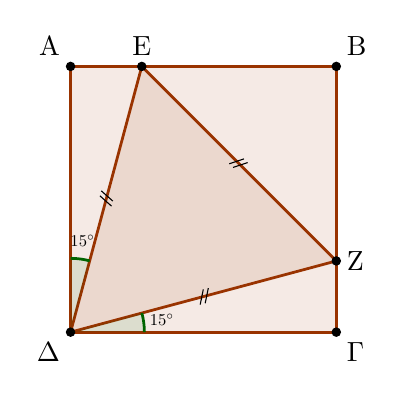
\begin{tikzpicture}[scale=.75]
\tkzSetUpLine[line width=1pt,color=black]
\tkzSetUpPoint[fill=black]

\tkzDefPoints{0/0/D,4.5/0/C,4.5/4.5/B,0/4.5/A}

\tkzDefPoint(15:0.5){x}
\tkzDefPoint(75:0.5){y}

\tkzInterLL(A,B)(D,y) \tkzGetPoint{E}
\tkzInterLL(B,C)(D,x) \tkzGetPoint{Z}

\tkzFillPolygon[fill=ShapeClr,fill opacity=0.1](A,B,C,D)
\tkzFillPolygon[fill=ShapeClr,fill opacity=0.1](D,E,Z)

\tkzDrawPolygon[color=ShapeClr](A,B,C,D)
\tkzDrawPolygon[color=ShapeClr](D,E,Z)

\tkzDrawPoints[size=3](A,B,C,D,E,Z)

\tkzFillAngles[fill=AngleClr,size=1.25,fill opacity=0.1](C,D,Z E,D,A)
\tkzMarkAngles[line width=1pt,size=1.25,color=AngleClr](C,D,Z E,D,A)
\tkzLabelAngles[scale=0.6,pos=2.6](C,D,Z E,D,A){$15^\circ$}

\tkzLabelPoint[above left](A){$\rm A$}
\tkzLabelPoint[above right](B){$\rm B$}
\tkzLabelPoint[below right](C){$\rm \Gamma$}
\tkzLabelPoint[below left](D){$\rm \Delta$}
\tkzLabelPoint[above](E){$\rm E$}
\tkzLabelPoint[right](Z){$\rm Z$}


\tkzMarkSegments[mark=s||,size=2.5](D,E Z,E D,Z)

\end{tikzpicture}

\end{document}
